%-----------------------------------
% Define document and include general packages
%-----------------------------------

\documentclass[12pt,oneside,titlepage,listof=totoc,bibliography=totoc]{scrartcl}
\usepackage[utf8]{inputenc}
%Dokumentensprache
\newif\ifde
\newif\ifen
 
%-----------------------------------
% Meta informationen
%-----------------------------------
%-----------------------------------
% Meta Informationen zur Arbeit
%-----------------------------------

% Autor
\newcommand{\myAutor}{Max Mustermann}

% Adresse
\newcommand{\myAdresse}{Heidestra\ss e 17 \\ \> \> \> 51147 Köln}

% Titel der Arbeit
\newcommand{\myTitel}{LATEX-Vorlage - mit Biblatex}

% Betreuer
\newcommand{\myBetreuer}{Prof. Dr. Peter Lustig}

% Lehrveranstaltung
\newcommand{\myLehrveranstaltung}{Modul Nr. 1}

% Matrikelnummer
\newcommand{\myMatrikelNr}{123456}

% Ort
\newcommand{\myOrt}{Düsseldorf}

% Datum der Abgabe
\newcommand{\myAbgabeDatum}{28. Februar 2014}

% Semesterzahl
\newcommand{\mySemesterZahl}{7}

% Name der Hochschule
\newcommand{\myHochschulName}{FOM Hochschule für Oekonomie \& Management Essen}

% Standort der Hochschule
\newcommand{\myHochschulStandort}{Düsseldorf}

% Studiengang
\newcommand{\myStudiengang}{Wirtschaftsinformatik}

% Art der Arbeit
\newcommand{\myThesisArt}{Bachelor Thesis}

% Zu erlangender akademische Grad
\newcommand{\myAkademischerGrad}{Bachelor of Science (B. Sc.)}

% Firma
\newcommand{\myFirma}{Mustermann GmbH}

%Deutsch
\detrue
\usepackage[ngerman]{babel}
%Englisch - Kommentar entfernen und die zwei Zeilen hierüber einkommentieren
%\entrue
%\usepackage[english]{babel}

\newcommand{\langde}[1]{%
   \ifde\selectlanguage{ngerman}#1\fi}
\newcommand{\langen}[1]{%
   \ifen\selectlanguage{english}#1\fi}
\usepackage[babel,german=quotes]{csquotes}
\usepackage[T1]{fontenc}
\usepackage{fancyhdr}
\usepackage{fancybox}
\usepackage[a4paper, left=4cm, right=2cm, top=2.8cm, bottom=2.3cm]{geometry}
\usepackage{graphicx}
\usepackage{colortbl}
\usepackage{array}
\usepackage{float}      %Positionierung von Abb. und Tabellen mit [H] erzwingen
\usepackage{footnote}
\usepackage{caption}
\usepackage{enumitem}
\usepackage{amssymb}
\usepackage{mathptmx}
\usepackage[scaled=0.9]{helvet} % Behebt, zusammen mit Package courier, pixelige Überschriften. Ist, zusammen mit mathptx, dem times-Package vorzuziehen. Details: https://latex-kurs.de/fragen/schriftarten/Times_New_Roman.html
\usepackage{courier}
\usepackage{amsmath}
\usepackage[table]{xcolor}
\usepackage{marvosym}			% Verwendung von Symbolen, z.B. perfektes Eurozeichen
\usepackage[colorlinks=true,linkcolor=black]{hyperref}
\definecolor{darkblack}{rgb}{0,0,0}
\hypersetup{colorlinks=true, breaklinks=true, linkcolor=darkblack, menucolor=darkblack, urlcolor=darkblack}
\fontfamily{ptm}\selectfont
\usepackage{ragged2e}

% Mehrere Fussnoten nacheinander mit Komma separiert
\usepackage[hang, multiple]{footmisc}
\setlength{\footnotemargin}{1em}

% todo Aufgaben als Kommentare verfassen für verschiedene Editoren
\usepackage{todonotes}

%Pakete für Tabellen
\usepackage{epstopdf}
\usepackage{nicefrac} % Brüche
\usepackage{multirow}
\usepackage{rotating} % vertikal schreiben
\usepackage{mdwlist}
\usepackage{tabularx}% für breitenangabe

\definecolor{dunkelgrau}{rgb}{0.8,0.8,0.8}
\definecolor{hellgrau}{rgb}{0.0,0.7,0.99}
% Colors for listings
\definecolor{mauve}{rgb}{0.58,0,0.82}
\definecolor{dkgreen}{rgb}{0,0.6,0}

% sauber formatierter Quelltext
\usepackage{listings}
\lstset{numbers=left,
	numberstyle=\tiny,
	numbersep=5pt,
	breaklines=true,
	showstringspaces=false,
	frame=l ,
	xleftmargin=5pt,
	xrightmargin=5pt,
	basicstyle=\ttfamily\scriptsize,
	stepnumber=1,
	keywordstyle=\color{blue},          % keyword style
  	commentstyle=\color{dkgreen},       % comment style
  	stringstyle=\color{mauve}         % string literal style
}

% Biblatex

%%%% Neuer Leitfaden (2018)
\usepackage[
backend=biber,
style=ext-authoryear,
maxcitenames=2,
maxbibnames=999,
mergedate=false,
date=iso,
urldate=iso,
innamebeforetitle,
dashed=false,
autocite=footnote,
doi=false
]{biblatex}%iso dateformat für YYYY-MM-DD

%weitere Anpassungen für BibLaTex
\usepackage{xpatch}

\setlength\bibhang{1cm}

%%% Weitere Optionen
%\boolitem[false]{citexref} %Wenn incollection, inbook, inproceedings genutzt wird nicht den zugehörigen parent auch in Literaturverzeichnis aufnehmen

%Aufräumen die Felder werden laut Leitfaden nicht benötigt.
\AtEveryBibitem{%
\ifentrytype{book}{
    \clearfield{issn}%
    \clearfield{doi}%
    \clearfield{isbn}%
    \clearfield{url}
    \clearfield{eprint}
}{}
\ifentrytype{collection}{
  \clearfield{issn}%
  \clearfield{doi}%
  \clearfield{isbn}%
  \clearfield{url}
  \clearfield{eprint}
}{}
\ifentrytype{incollection}{
  \clearfield{issn}%
  \clearfield{doi}%
  \clearfield{isbn}%
  \clearfield{url}
  \clearfield{eprint}
}{}
\ifentrytype{article}{
  \clearfield{issn}%
  \clearfield{doi}%
  \clearfield{isbn}%
  \clearfield{url}
  \clearfield{eprint}
}{}
\ifentrytype{inproceedings}{
  \clearfield{issn}%
  \clearfield{doi}%
  \clearfield{isbn}%
  \clearfield{url}
  \clearfield{eprint}
}{}
}

\renewcommand*{\finentrypunct}{}%Kein Punkt am ende des Literaturverzeichnisses

\renewcommand*{\newunitpunct}{\addcomma\space}
\DeclareDelimFormat[bib,biblist]{nametitledelim}{\addcolon\space}
\DeclareDelimFormat{titleyeardelim}{\newunitpunct}
%Namen kursiv schreiben
\renewcommand*{\mkbibnamefamily}{\mkbibemph}
\renewcommand*{\mkbibnamegiven}{\mkbibemph}
\renewcommand*{\mkbibnamesuffix}{\mkbibemph}
\renewcommand*{\mkbibnameprefix}{\mkbibemph}

% Die Trennung mehrerer Autorennamen erfolgt durch Kommata.
% siehe Beispiele im Leitfaden S. 16
% Die folgende Zeile würde mit Semikolon trennen
%\DeclareDelimFormat{multinamedelim}{\addsemicolon\addspace}

%Delimiter für mehrere und letzten Namen gleich setzen
\DeclareDelimAlias{finalnamedelim}{multinamedelim}

\DeclareNameAlias{default}{family-given}
\DeclareNameAlias{sortname}{default}  %Nach Namen sortieren


\DeclareFieldFormat{editortype}{\mkbibparens{#1}}
\DeclareDelimFormat{editortypedelim}{\addspace}
\DeclareFieldFormat{translatortype}{\mkbibparens{#1}}
\DeclareDelimFormat{translatortypedelim}{\addspace}
\DeclareDelimFormat[bib,biblist]{innametitledelim}{\addcomma\space}

\DeclareFieldFormat*{citetitle}{#1}
\DeclareFieldFormat*{title}{#1}
\DeclareFieldFormat*{booktitle}{#1}
\DeclareFieldFormat*{journaltitle}{#1}

\xpatchbibdriver{online}
  {\usebibmacro{organization+location+date}\newunit\newblock}
  {}
  {}{}

\DeclareFieldFormat[online]{date}{\mkbibparens{#1}}
\DeclareFieldFormat{urltime}{\addspace #1\addspace \langde{Uhr}\langen{MEZ}}
\DeclareFieldFormat{urldate}{%urltime zu urldate hinzufügen
  [\langde{Zugriff}\langen{Access}\addcolon\addspace
  #1\printfield{urltime}]
}
\DeclareFieldFormat[online]{url}{<\url{#1}>}
\renewbibmacro*{url+urldate}{%
  \usebibmacro{url}%
  \ifentrytype{online}
    {\setunit*{\addspace}%
     \iffieldundef{year}
       {\printtext[date]{\langde{keine Datumsangabe}\langen{no Date} }}
       {\usebibmacro{date}}}%
    {}%
  \setunit*{\addspace}%
  \usebibmacro{urldate}
  }

%Verhindern, dass bei mehreren Quellen des gleichen Autors im gleichen Jahr
%Buchstaben nach der Jahreszahl angezeigt werden wenn sich das Keyword in usera unterscheidet.
\DeclareExtradate{
  \scope{
    \field{labelyear}
    \field{year}
    }
    \scope{
      \field{usera}
     }
}

%% Anzeige des Jahres nach dem Stichwort (usera) im Literaturverzeichnis
%% Wenn das Jahr bei Online-Quellen nicht explizit angegeben wurde, wird nach
%% dem Stichwort 'o. J.' ausgegeben. Nach der URL steht dann 'keine
%% Datumsangabe'. Ist das Jahr definiert, wird es an beiden Stellen ausgegeben.
%% Das Zugriffsdatum (urldate) spielt hier keine Rolle.
%% Für Nicht-Online-Quellen wird nichts geändert.
\renewbibmacro*{date+extradate}{%
  \printtext[parens]{%
    \printfield{usera}%
    \setunit{\printdelim{titleyeardelim}}%
    \ifentrytype{online}
       {\setunit*{\addspace\addcomma\addspace}%
         \iffieldundef{year}
           {\bibstring{nodate}}
       {\printlabeldateextra}}%
       {\printlabeldateextra}}}

%% Anzeige des Jahres nach dem Stichwort (usera) in der Fussnote
%% das Stichwort hat der Aufrufer hier schon ausgegeben.
%% siehe auch Kommentar zu: \renewbibmacro*{date+extradate}
\renewbibmacro*{cite:labeldate+extradate}{%
    \ifentrytype{online}
       {\setunit*{\addspace\addcomma\addspace}%
         \iffieldundef{year}
           {\bibstring{nodate}}
       {\printlabeldateextra}}%
       {\printlabeldateextra}}


\DefineBibliographyStrings{german}{
  nodate    = {{}o.\adddot\addspace J\adddot},
  andothers = {et\addabbrvspace al\adddot}
}
\DefineBibliographyStrings{english}{
  nodate    = {{}n.\adddot\addspace d\adddot},
  andothers = {et\addabbrvspace al\adddot}
}
\DeclareSourcemap{
  \maps[datatype=bibtex]{
    \map{
      \step[notfield=translator, final]
      \step[notfield=editor, final]
      \step[fieldset=author, fieldvalue={{{\langde{o\noexpand\adddot\addspace V\noexpand\adddot}\langen{Anon}}}}]
    }
    \map{
      \pernottype{online}
      \step[fieldset=location, fieldvalue={\langde{o\noexpand\adddot\addspace O\noexpand\adddot}\langen{s\noexpand\adddot I\noexpand\adddot}}]
    }
  }
}

\renewbibmacro*{cite}{%
  \iffieldundef{shorthand}
    {\ifthenelse{\ifnameundef{labelname}\OR\iffieldundef{labelyear}}
       {\usebibmacro{cite:label}%
        \setunit{\printdelim{nonametitledelim}}}
       {\printnames{labelname}%
        \setunit{\printdelim{nametitledelim}}}%
     \printfield{usera}%
     \setunit{\printdelim{titleyeardelim}}%
     \usebibmacro{cite:labeldate+extradate}}
    {\usebibmacro{cite:shorthand}}}

    \renewcommand*{\jourvoldelim}{\addcomma\addspace}% Trennung zwischen journalname und Volume. Sonst Space; Laut Leitfaden richtig
    %Aufgrund der Änderung bzgl des Issues 169 in der thesis_main.tex musste ich die Zeile auskommentieren. Konnte aber das Verhalten, dass die Fußnoten grün sind, im nachhinein nicht feststellen.
    %\hypersetup{hidelinks} %sonst sind Fußnoten grün. Dadurch werden Links allerdings nicht mehr farbig dargestellt

\renewbibmacro*{journal+issuetitle}{%
  \usebibmacro{journal}%
  \setunit*{\jourvoldelim}%
  \iffieldundef{series}
    {}
    {\setunit*{\jourserdelim}%
     \printfield{series}%
     \setunit{\servoldelim}}%
  \iffieldundef{volume}
    {}
    {\printfield{volume}}
  \iffieldundef{labelyear}
  {}
  {
  (\thefield{year}) %Ansonsten wird wenn kein Volume angegeben ist ein Komma vorangestellt
  }
  \setunit*{\addcomma\addspace Nr\adddot\addspace}
  \printfield{number}
  \iffieldundef{eid}
  {}
  {\printfield{eid}}
}

% Postnote ist der Text in der zweiten eckigen Klammer bei einem Zitat
% wenn es keinen solchen Eintrag gibt, dann auch nicht ausgeben, z.B. 'o. S.'
% Wenn man das will, kann man das 'o. S.' ja explizit angeben. Andernfalls steht
% sonst auch bei Webseiten 'o. S.' da, was laut Leitfaden nicht ok ist.
\renewbibmacro*{postnote}{%
  \setunit{\postnotedelim}%
  \iffieldundef{postnote}
    {} %{\printtext{\langde{o.S\adddot}\langen{no page number}}}
    {\printfield{postnote}}}

% Abstand bei Änderung Anfangsbuchstabe ca. 1.5 Zeilen
\setlength{\bibinitsep}{0.75cm}

% nur in den Zitaten/Fussnoten den Vornamen abkürzen (nicht im
% Literaturverzeichnis)

\DeclareDelimFormat{nonameyeardelim}{\addcomma\space}
\DeclareDelimFormat{nameyeardelim}{\addcomma\space}

\renewbibmacro*{cite}{%
  \iffieldundef{shorthand}
    {\ifthenelse{\ifciteibid\AND\NOT\iffirstonpage}
       {\usebibmacro{cite:ibid}}
    {\ifthenelse{\ifnameundef{labelname}\OR\iffieldundef{labelyear}}
       {\usebibmacro{cite:label}%
        \setunit{\printdelim{nonameyeardelim}}}
      {\toggletrue{abx@bool@giveninits}%
        \printnames[family-given]{labelname}%
        \setunit{\printdelim{nameyeardelim}}}%
      \printfield{usera}%
      \setunit{\printdelim{titleyeardelim}}%
     \usebibmacro{cite:labeldate+extradate}}}
   {\usebibmacro{cite:shorthand}}}


%%%%% Alter Leitfaden. Ggf. Einkommentieren und Bereich hierüber auskommentieren
%\usepackage[
%backend=biber,
%style=numeric,
%citestyle=authoryear,
%url=false,
%isbn=false,
%notetype=footonly,
%hyperref=false,
%sortlocale=de]{biblatex}

%weitere Anpassungen für BibLaTex
%% Opptionen für Biblatex
\ExecuteBibliographyOptions{%
firstinits=false,
isbn=true, 
url=true, 
doi=false, 
eprint=false,
maxbibnames=7, % Alle Autoren (kein et al.)
maxcitenames=1, % Kürzel nur aus 1. Autor
backref=false, % Rückverweise auf Zitatseiten
bibencoding=utf8, % wenn .bib in utf8, sonst ascii
bibwarn=true, % Warnung bei fehlerhafter bib-Datei
}%

% et al. an Stelle von u.a.
\DefineBibliographyStrings{ngerman}{ 
   andothers = {{et\,al\adddot}},             
}

% Klammern um das Jahr in der Fußnote
\renewbibmacro*{cite:labelyear+extrayear}{% 
  \iffieldundef{labelyear} 
    {} 
    {\printtext[bibhyperref]{% 
       \mkbibparens{% 
         \printfield{labelyear}% 
         \printfield{extrayear}}}}}

\DeclareNameFormat{last-first}{%
  \iffirstinits
    {\usebibmacro{name:last-first}{#1}{#4}{#5}{#7}}
    {\usebibmacro{name:last-first}{#1}{#3}{#5}{#7}}%
  \usebibmacro{name:andothers}}

%Autoren (Nachname, Vorname)
\DeclareNameAlias{default}{last-first}

%Reihenfolge von publisher, year, address verändern
% Achtung, bisher nur für den Typ @book definiert

%% Definiert @Book Eintrag
\DeclareBibliographyDriver{book}{%
  \printnames{author}%
  \newunit\addcolon\space
  \printfield{title}%
  \setunit*{,\space}%
  \printfield{edition}%
  \setunit*{\addcomma\space}%
  \printlist{publisher}%
  \newunit\newblockpunct
  \printlist{location}%
  \setunit*{\space}%
  \printfield{year}%
  \setunit*{,\space}% 
  \printfield{isbn}%
  \finentry}

%% Definiert @Online Eintrag
\DeclareBibliographyDriver{online}{%
  \printnames{author}%
  \newunit\newblockpunct
  \printfield{title}%
  \setunit*{.\space}%
  %\newunit\newblock
  \printfield{url}%
  \setunit*{.\space}%
  \printfield{note}%
  \finentry}
  
%% Definiert @Article Eintrag
\DeclareBibliographyDriver{article}{%
  \printnames{author}%
  \newunit\newblockpunct
  \printfield{title}%
  \setunit*{.\space In:\space}%
  %\newunit\newblock
  \usebibmacro{journal}%
  \setunit*{\space (}%
  \printfield{year}\newunit{)}%
  \finentry}  

%Doppelpunkt nach dem letzten Autor
\renewcommand*{\labelnamepunct}{\addcolon\addspace }

%Komma an Stelle des Punktes
\renewcommand*{\newunitpunct}{\addcomma\space}

%Autoren durch Semikolon trennen
\newcommand*{\bibmultinamedelim}{\addsemicolon\space}% 
\newcommand*{\bibfinalnamedelim}{\addsemicolon\space}% 
\AtBeginBibliography{% 
  \let\multinamedelim\bibmultinamedelim 
  \let\finalnamedelim\bibfinalnamedelim 
}

%Titel nicht kursiv anzeigen 
\DeclareFieldFormat{title}{#1\isdot}

%%%% Ende Alter Leitfaden

%Bib-Datei einbinden
\addbibresource{literatur/literatur.bib}

% Pfad fuer Abbildungen
\graphicspath{{./}{./abbildungen/}}

%-----------------------------------
% Weitere Ebene einfügen
\usepackage{titletoc}

\makeatletter

% Setze die Tiefe des Inhaltsverzeichnis auf 4 Ebenen
% Damit erscheinen \paragraph-Sektionen auch im Inhaltsverzeichnis
\setcounter{secnumdepth}{4}
\setcounter{tocdepth}{4}

% Fuege Abstand nach unten wie in einer normalen \section hinzu
% Andernfalls haette \paragraph keinen Zeilenumbruch
% Der Zeilenumbruch koennte mit einer leeren \mbox{} ersetzt werden
% Jedoch klebt dann der Text relativ nah an der Ueberschrift
\renewcommand{\paragraph}{%
  \@startsection{paragraph}{4}%
  {\z@}{3.25ex \@plus 1ex \@minus .2ex}{1.5ex plus 0.2ex}%
  {\normalfont\normalsize\bfseries\sffamily}%
}

\makeatother


%-----------------------------------
% Zeilenabstand 1,5-zeilig
%-----------------------------------
\usepackage{setspace}
\onehalfspacing

%-----------------------------------
% Absätze durch eine neue Zeile
%-----------------------------------
\setlength{\parindent}{0mm}
\setlength{\parskip}{0.8em plus 0.5em minus 0.3em}

\sloppy					%Abstände variieren
\pagestyle{headings}

%-----------------------------------
% Abkürzungsverzeichnis
%-----------------------------------
\usepackage[intoc]{nomencl}
\renewcommand{\nomname}{Abkürzungsverzeichnis}
\setlength{\nomlabelwidth}{.20\textwidth}
\renewcommand{\nomlabel}[1]{#1 \dotfill}
\setlength{\nomitemsep}{-\parsep}
\makenomenclature

%-----------------------------------
% PDF Meta Daten setzen
%-----------------------------------
\hypersetup{
    pdfinfo={
        Title={\myTitel},
        Subject={\myStudiengang},
        Author={\myAutor},
        Build=1.1
    }
}

%-----------------------------------
% Umlaute in Code korrekt darstellen
% siehe auch: https://en.wikibooks.org/wiki/LaTeX/Source_Code_Listings
%-----------------------------------
\lstset{literate=
	{á}{{\'a}}1 {é}{{\'e}}1 {í}{{\'i}}1 {ó}{{\'o}}1 {ú}{{\'u}}1
	{Á}{{\'A}}1 {É}{{\'E}}1 {Í}{{\'I}}1 {Ó}{{\'O}}1 {Ú}{{\'U}}1
	{à}{{\`a}}1 {è}{{\`e}}1 {ì}{{\`i}}1 {ò}{{\`o}}1 {ù}{{\`u}}1
	{À}{{\`A}}1 {È}{{\'E}}1 {Ì}{{\`I}}1 {Ò}{{\`O}}1 {Ù}{{\`U}}1
	{ä}{{\"a}}1 {ë}{{\"e}}1 {ï}{{\"i}}1 {ö}{{\"o}}1 {ü}{{\"u}}1
	{Ä}{{\"A}}1 {Ë}{{\"E}}1 {Ï}{{\"I}}1 {Ö}{{\"O}}1 {Ü}{{\"U}}1
	{â}{{\^a}}1 {ê}{{\^e}}1 {î}{{\^i}}1 {ô}{{\^o}}1 {û}{{\^u}}1
	{Â}{{\^A}}1 {Ê}{{\^E}}1 {Î}{{\^I}}1 {Ô}{{\^O}}1 {Û}{{\^U}}1
	{œ}{{\oe}}1 {Œ}{{\OE}}1 {æ}{{\ae}}1 {Æ}{{\AE}}1 {ß}{{\ss}}1
	{ű}{{\H{u}}}1 {Ű}{{\H{U}}}1 {ő}{{\H{o}}}1 {Ő}{{\H{O}}}1
	{ç}{{\c c}}1 {Ç}{{\c C}}1 {ø}{{\o}}1 {å}{{\r a}}1 {Å}{{\r A}}1
	{€}{{\EUR}}1 {£}{{\pounds}}1 {„}{{\glqq{}}}1
}

%-----------------------------------
% Kopfbereich / Header definieren
%-----------------------------------
\pagestyle{fancy}
\fancyhf{}
\fancyhead[C]{-\ \thepage\ -}						% Seitenzahl oben, mittg
%\fancyhead[L]{\leftmark}							% kein Footer vorhanden
\renewcommand{\headrulewidth}{0.4pt}


%-----------------------------------
% Start the document here:
%-----------------------------------
\begin{document}

\pagenumbering{Roman}								% Seitennumerierung auf römisch umstellen
\renewcommand{\refname}{\langde{Literaturverzeichnis}
						\langen{Bibliography}}		% "Literatur" in
%"Literaturverzeichnis" umbenennen
\newcolumntype{C}{>{\centering\arraybackslash}X}	% Neuer Tabellen-Spalten-Typ:
%Zentriert und umbrechbar

%-----------------------------------
% Titlepage
%-----------------------------------
\begin{titlepage}
	\newgeometry{left=2cm, right=2cm, top=2cm, bottom=2cm}
	\begin{center}
		\textbf{\myHochschulName}\\
		\textbf{
			\langde{Hochschulzentrum}
			\langen{university location}
			\myHochschulStandort}\\
		\vspace{1.5cm}
			
\includegraphics[width=3cm]{abbildungen/fomLogo.jpg} \\
		\vspace{1.5cm}
		\langde{Berufsbegleitender Studiengang}
		\langen{part-time degree program}\\
		\myStudiengang, \mySemesterZahl. Semester\\
		\vspace{2cm}
		\textbf{\myThesisArt}\\
		\textbf{
				\langde{zur Erlangung des Grades eines}
				\langen{to obtain the degree of}
				}\\
		\textbf{\myAkademischerGrad}\\
		% Oder für Hausarbeiten:
		%\textbf{im Rahmen der Lehrveranstaltung}\\
		%\textbf{\myLehrveranstaltung}\\
		\vspace{2cm}
		\langde{über das Thema}
		\langen{on the subject}\\
		\Huge{\myTitel}\\
		\vspace{0.2cm}
	\end{center}
	\normalsize
	\vfill
	\begin{tabbing}
		Links \= Mitte \=Mittez \= Rechts\kill
		\langde{Betreuer}
		\langen{Advisor}: \> \> \>\myBetreuer\\
		\> \> \\

		\langde{Autor}
		\langen{Author}: \> \> \> \myAutor\\
		\> \> \>  \langde{Matrikelnr.}
				\langen{Matriculation Number}: \myMatrikelNr\\
		\> \> \> \myAdresse\\
		\> \> \>  \\
		\langde{Abgabe}
		\langen{Submission}: \> \> \> \myAbgabeDatum
	\end{tabbing}
\end{titlepage}

%-------Ende Titelseite-------------

%-----------------------------------
% Sperrvermerk
%-----------------------------------
%\newpage
\thispagestyle{empty}

%-----------------------------------
% Sperrvermerk
%-----------------------------------
\section*{Sperrvermerk}
Die vorliegende Abschlussarbeit mit dem Titel \enquote{\myTitel} enthält unternehmensinterne Daten der Firma \myFirma . Daher ist sie nur zur Vorlage bei der FOM sowie den Begutachtern der Arbeit bestimmt. Für die Öffentlichkeit und dritte Personen darf sie nicht zugänglich sein.

\par\medskip
\par\medskip

\_\_\_\_\_\_\_\_\_\_\_\_\_\_\_\_\_\_\_\_\_\_\_\_ \hspace{1.5cm} \_\_\_\_\_\_\_\_\_\_\_\_\_\_\_\_\_\_\_\_\_\_\_\_ \\
(Ort, Datum)\hspace{4.5cm}
(Eigenhändige Unterschrift)

\newpage

%-----------------------------------
% Inhaltsverzeichnis
%-----------------------------------
\setcounter{page}{2}
\tableofcontents
\newpage
\setcounter{tocdepth}{2} %wurde vorher in zusaetzlichesMaterial.tex auf 0 gesetzt um Inhalt des Anhangs zu verbergen. Dadurch gehen allerdings Abbildungs und Tabellenverzeichnis kaputt.

%-----------------------------------
% Abkürzungsverzeichnis
%-----------------------------------
\printnomenclature
\newpage
%-----------------------------------
% Abbildungsverzeichnis
%-----------------------------------
\listoffigures
\newpage
%-----------------------------------
% Tabellenverzeichnis
%-----------------------------------
\listoftables
\newpage
%-----------------------------------
% Seitennummerierung auf arabisch und ab 1 beginnend umstellen
%-----------------------------------
\pagenumbering{arabic}
\setcounter{page}{1}
%-----------------------------------
% Kapitel / Inhalte
%-----------------------------------
\section{Einleitung}
Dies soll eine \LaTeX{}-Vorlage für den persönlichen Gebrauch werden. Sie hat weder einen Anspruch auf Richtigkeit, noch auf Vollständigkeit. Die Quellen liegen auf Github zur allgemeinen Verwendung. Verbesserungen sind jederzeit willkommen. 

\subsection{Zielsetzung}
Kleiner Reminder für mich in Bezug auf die Dinge, die wir bei der Thesis beachten sollten und \LaTeX{}-Vorlage für die Thesis.

\subsection{Aufbau der Arbeit}
Kapitel \ref{infos} enthält die Inhalte des Thesis-Days und alles, was zum inhaltlichen erstellen der Thesis relevant sein könnte. In Kapitel \ref{latexDetails} \nameref{latexDetails} findet ihr wichtige Anmerkungen zu \LaTeX{}, wobei die wirklich wichtigen Dinge im Quelltext dieses Dokumentes stehen.

\begin{figure}[H]
\begin{center}

\includegraphics[width=0.9\textwidth]{verzeichnisStruktur}
\caption{Verzeichnisstruktur der \LaTeX{}-Datein}
\end{center}
\end{figure}

\newpage
\section{Informationen vom Thesis-Day} \label{infos}
Siehe auch Wissenschaftliches Arbeiten~\footcite[Vgl. ][S. 1]{Balzert.2008}. Damit sollten alle wichtigen Informationen abgedeckt sein ;-)

\subsection{Pre-Anmeldephase}
\subsubsection{Vorüberlegungen}
Trichtermethode: Man beginnt mit der eigentlichen  Konklusion und überlegt dann, welche allgemeinen Teile dafür benötigt werden. 

Welchen Mehrwert soll die Arbeit bieten \footnote{Diese Fußnote hat inhaltlich keinen Sinn. Es soll nur ein langer Text generiert werden, dass dieser Vermerk über zwei Zeilen reicht und bündig dargestellt wird.}? Auch darüber nachdenken, wie die Arbeit einen selbst weiter bringen kann. Studienverlauf prüfen. Welche Vorlesungen hat mich besonders interessiert? Wo liegen meine Stärken etc.

\begin{enumerate}
\item Themenfindung
\item Literaturrecherche
\item Gliederung/Motivationspapier erstellen
\item Betreuerauswahl (siehe Liste im \nomenclature{OC}{FOM Online Campus} OC)
\item Anmeldung (ab 141 Credits möglich)
\end{enumerate}

\subsubsection{Anregungen finden}
\begin{itemize}
\item \href{http://www.diplom.de}{www.diplom.de}
\item \href{http://www.hausarbeiten.de}{www.hausarbeiten.de}
\item Datenbanken aus Tools and Methods
\item etc.
\end{itemize}

\newpage
\subsection{Anfertigungsphase}
Die Anmeldung ist mittlerweile jeden Mittwoch möglich. 
\begin{figure}[H]
\begin{center}
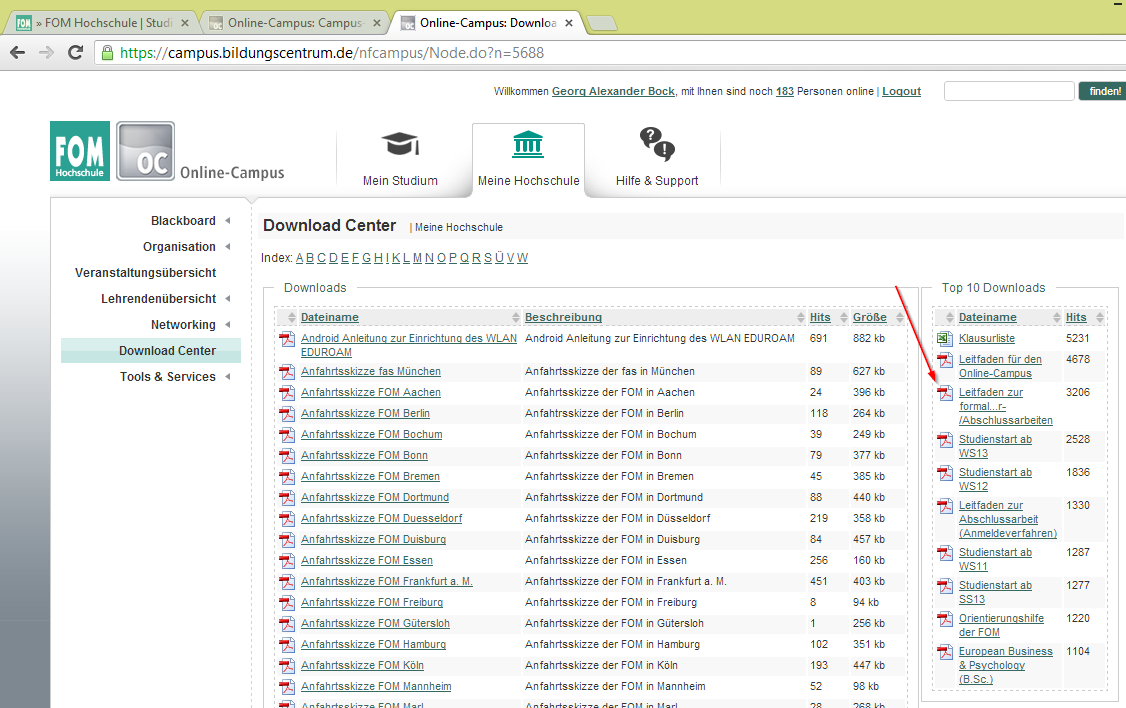
\includegraphics[width=0.9\textwidth]{campusDownload}
\caption{FOM-Vorgaben zur Thesis im Online-Campus}
\end{center}
\end{figure}

Laut Herrn Keller sollte der Umfang der Thesis (für eine gute Note) eher im Bereich der 60 Seiten liegen. Wie immer ist das vermutlich mit dem Betreuer abzustimmen. Die Liste der Dozenten, die Abschlussarbeiten betreuen, findet sich auch im OC.

Zeit zur Erstellung der Thesis 2-4 Monate.

Es müssen zwei gedruckte Arbeiten abgegeben werden. Flüchtige Quellen als PDF ausgeben lassen und auf CD abgeben. Thesis zusätzlich digital einreichen. Beim Binden der Thesis auf Qualität achten. Haptik und erster Eindruck sind in der Bewertung \enquote{auch} wichtig. Arbeiten können in jedem FOM Studienzentrum abgegeben werden. 

\subsection{Post-Abgabephase}
Nach Abgabe ca. 2 Wochen bis zum Kolloquium.

Kolloquium:
\begin{itemize}
\item Dauer: 30 Minuten 
\item Präsentation (manche Prüfer wollen eine, andere nicht)
\item Betreuer vorher fragen was er möchte
\item Es gibt einen Frageteil, dieser bezieht sich auf die Arbeit, kann aber auch darüber hinaus gehen.
\item Der Tag des Kolloquiums steht auf der Endbenotung 
\item Thesis und Kolloquium sind zwei getrennte Prüfungsbereiche. Für beide gibt es nur zwei Versuche. 
\item Am Tag des Kolloquiums erhält man die Bestätigung, ob bestanden oder nicht
\end{itemize}

\newpage
\section{Latex-Details} \label{latexDetails}

\subsection{Verwendete Software, Editor und Zusatzpakete}
\subsubsection{Windows 8+}
\begin{itemize}
\item MikTex: 2.9, 32-bit
\item Biblatex: 3.5, Zusatz: Biber.exe
\item Editor: TexStudio (kann ich empfehlen), Notepad++
\end{itemize}

\subsubsection{Mac OSX und iOS}
\begin{itemize}
\item MacTeX: \url{https://tug.org/mactex}
\item Editor: TexPad \url{https://www.texpadapp.com}
\end{itemize}

\subsubsection{Online}
Overleaf ist eine Online-Anwendung mit der Ihr direkt im Browser an eurer Thesis schreiben könnt. Bis 1GB Größe und maximal 60 Einzeldateien könnt ihr Overleaf kostenlos nutzen: \url{https://www.overleaf.com/}


\subsection{Dokumentenklasse}
Eigentlich hatte Prof. Finke empfohlen die Dokumentklassen \enquote{Book} oder \enquote{Report} für die Erstellung der Bachelor-Thesis zu verwenden, da diese über weitere Gliederungsebenen verfügen. Ich verwende dennoch eine leicht modifizierte Komaskript-Klasse \enquote{scrartcl}, mit der Erweiterung um eine Ebene. Siehe (skripte/weitereEbene.tex). Das Skript stammt irgendwo aus den Netz und übersteigt meine \LaTeX{}-Fähigkeiten. Dadurch kann ich über eine weitere Ebene in der Arbeit verfügen, ohne mich mit der Modifikation von Kapitel-Seiten rumschlagen~\footcite[Vgl. ][S. 5]{Tanenbaum.2003} zu müssen. Diese Quelle ist nur zur Demonstration und hat keinen inhaltlichen Bezug hierzu. Es werden übrigens nur die Quellen im Literaturverzeichnis angezeigt, die auch referenziert sind.


\subsection{Grafiken}
Das Paket \textbackslash usepackage\{float\} ermöglicht es die Grafiken und Tabellen an der Stelle im Text zu positionieren, wo diese im Quelltext stehen (Option H). Ansonsten würde \LaTeX{} diese dort unterbringen, wo es typographisch sinnvoll wäre - das wollen wir ja nicht ;-).

Die Breite der Grafiken am Besten relativ zum Text angeben.

\subsection{Quellcode}
Quellcode kann auf unterschiedliche Arten eingebaut werden.
Zum einen kann es hier durch direktives Einbinden in der Kapitel-Datei geschehen.
\begin{lstlisting}
% Hier wird aufgezeigt, wie man eine Grafik einbindet, es wird also in der PDF angezeigt,
% da es in einem Quellcode-Listing steht.
% Auch wenn es hier faelschlicherweise als LaTeX-Befehl angezeigt wird.
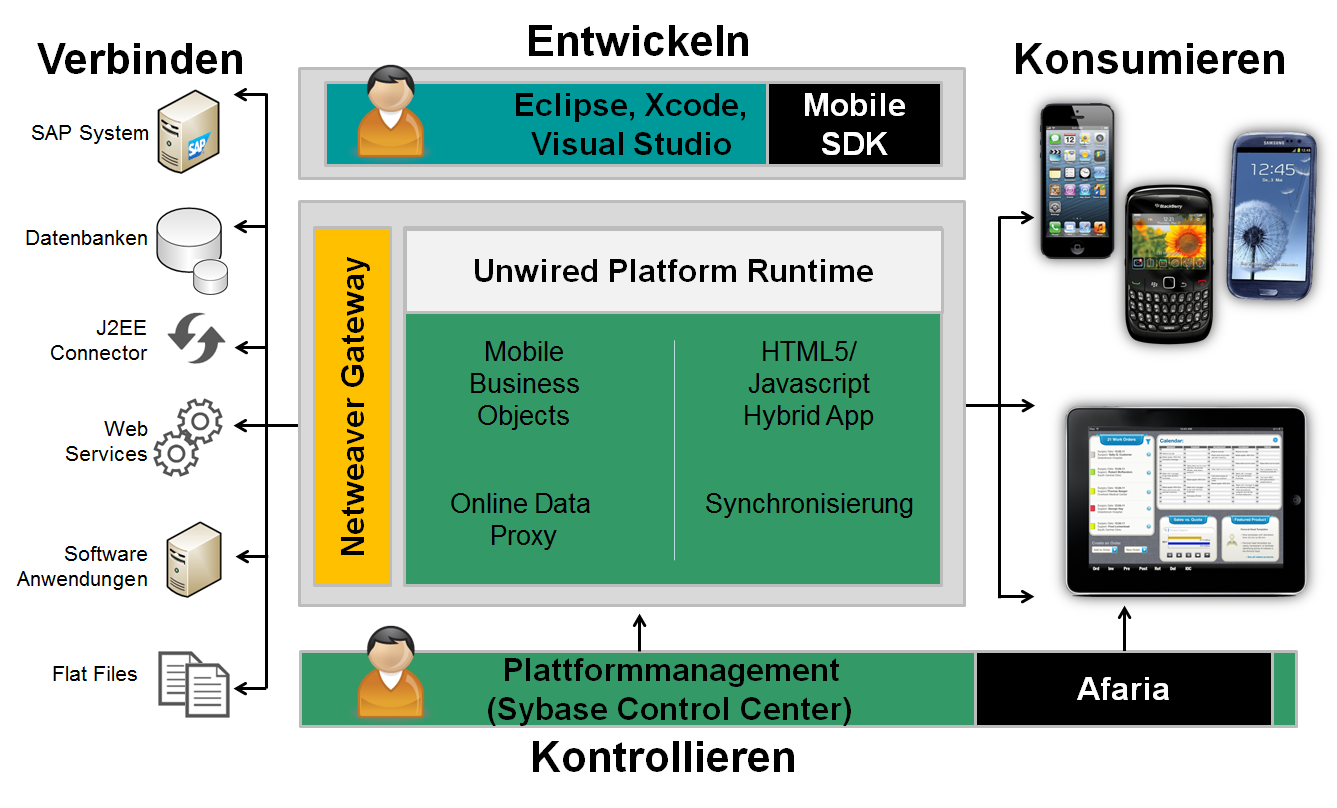
\includegraphics[width=0.9\textwidth]{sup}
\end{lstlisting}

Bei längeren Quellcode-Listings empfiehlt es sich jedoch auf eine externe Datei im Ordner Quellcode zu verlinken und diese einzubauen:
\lstinputlisting[language=HTML]{./Quellcode/Beispiel.html}

Statt dem Package lstlisting, welches direkt auf Tex basiert, kann auch das Package minted verwendet werden.
Dieses Package basiert auf python-pygments und unterstützt weit mehr Sprachkonstrukte als lstlisting.
Um das Paket zu verwenden muss es eingebunden werden und zusätzlich python-pygments installiert sein.
(Dies ist mit im Dockerfile vorhanden. Für die anderen Compile-Methoden, wie das native verwenden von Tex Live findet sich hier die Installationsanleitung für das minted Paket: https://ctan.org/pkg/minted?lang=de)

Damit das kompilieren ohne Python trotzdem möglich ist, ist die Funktion standardmäßig ausgebaut. Deshalb muss zusätzlich in der Datei \begin{verbatim}thesis_main.tex \usepackage{minted} \end{verbatim} wieder einkommentiert werden. 

Minted lässt sich dann ganz ähnlich zu lstlisting verwenden:
\begin{lstlisting}
	\begin{minted}{c}
		int main() {
			printf("hello, world");
			return 0;
		}
	\end{minted}
\end{lstlisting}	

Da der Pfad zu den Abbildungen im Hauptdokument definiert wurde, muss hier nur noch der Name des Bildes ohne Dateiendung stehen (sup).

\begin{figure}[H]
\caption{Titel der Abbildung hier}
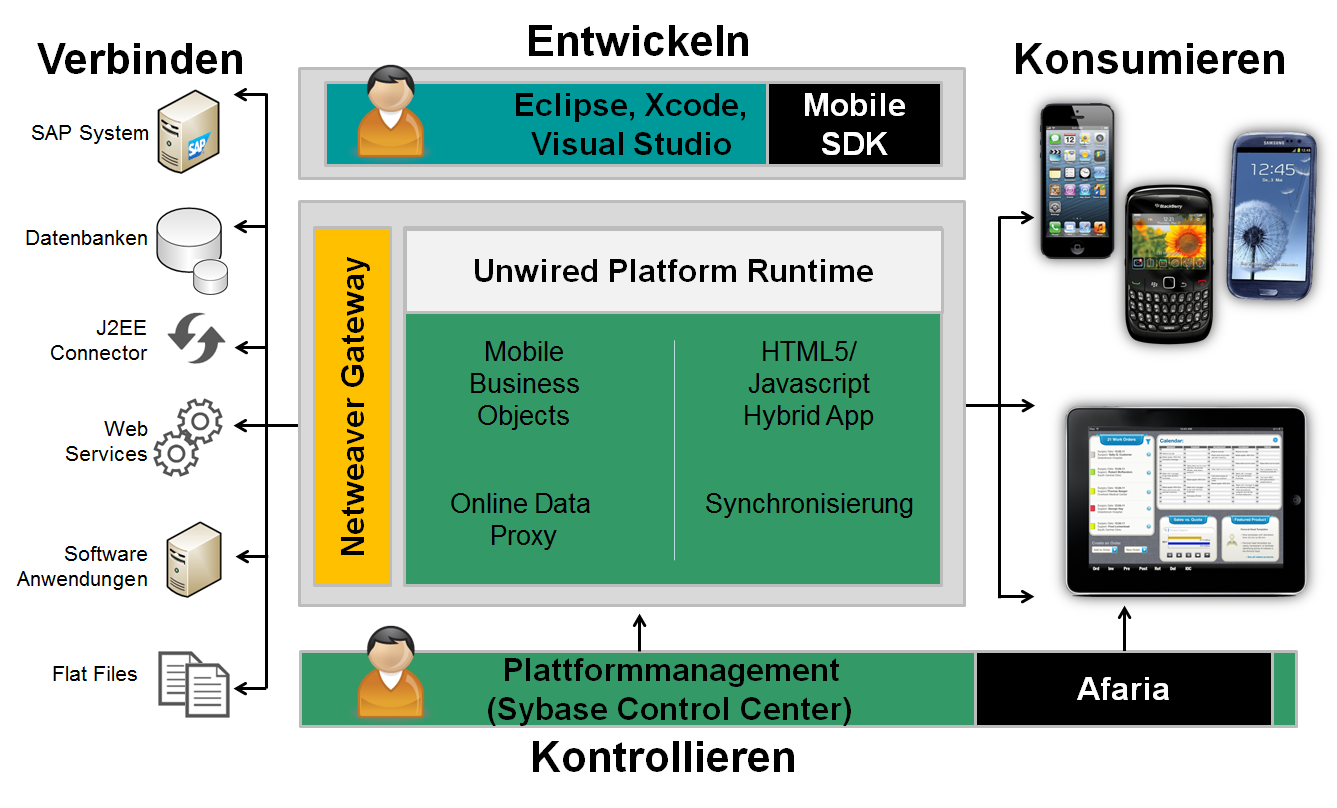
\includegraphics[width=0.9\textwidth]{sup}
\\
Quelle: Eigene Darstellung
\end{figure}

\subsection{Tabellen}
\begin{table}[H]
\caption{Beispieltabelle 1}
\label{tbl:beispieltabelle2}
\begin{tabularx}{\textwidth}[ht]{|l|X|l|}
  \hline
  \textbf{Abkürzung} & \textbf{Beschreibung} & \textbf{Berechnung}\\
  \hline\hline
    MEK & Materialeinzelkosten & \\
  	MGK & Materialgemeinkosten & $+ \uparrow$~*\\
    FEK & Fertigungseinzelkosten & \\
  	FGK & Fertigungsgemeinkosten & $+ \uparrow$~*\\
	SEKF & Sondereinzelkosten der Fertigung & \\
	\hline\hline
	\multicolumn{3}{|l|}{\textbf{= Herstellungskosten}} \\
	\hline\hline
  	VwGK & Verwaltungsgemeinkosten & $+ \uparrow$~*\\
  	VtGK & Vertriebsgemeinkosten & $+ \uparrow$~*\\
  	SEKVt & Sondereinzelkosten des Vertriebes & \\
	\hline\hline
	\multicolumn{3}{|l|}{\textbf{= Selbstkosten}} \\
	\hline\hline
	\multicolumn{3}{|l|}{+ Gewinnaufschlag} \\
	\multicolumn{3}{|l|}{+ Rabatte} \\
	\hline\hline
	\multicolumn{3}{|l|}{\textbf{= Nettoverkaufspreis (NVP)}} \\
	\hline
	\multicolumn{3}{|l|}{+ Umsatzsteuer} \\
	\hline\hline
	\multicolumn{3}{|l|}{\textbf{= Bruttoverkaufspreis (BVP)}} \\
	\hline
\end{tabularx} \\
\cite[Quelle: In Anlehnung an][S. 4]{Beckert.2012}
\end{table}

%\clearpage % hiermit werden alle Bilder Tabellen ausgeworfen

\subsection{Biblatex}
Von den vielen verfügbaren Literatur-Paketen habe ich mich für Biblatex entschieden. Die Anforderungen der FOM sollten hiermit erfüllt sein. Ich habe bisher nur Einträge \enquote{@book} getestet. Wie immer steckt der Teufel hier im Detail und es wird sich später herausstellen, ob Biblatex eine gute Wahl war. Die Anpassungen hierfür liegen unter skripte/modsBiblatex. Ich verwende das Backend Biber, welches bib-Dateien in UTF-8 verarbeiten kann.

In der für den Leitfaden 2018 aktualisierten Version sind außerdem Beispiele für \enquote{online},\footcite[Vgl.][]{website:angular:aboutAngular} also Webseiten, und \enquote{article},\footcite[Vgl.][S. 140]{Decker2009} also wissenschaftliche Artikel, enthalten.

Laut Leitfaden sollen maximal 3 Autoren genannt werden und danach mit
\enquote{et.
al.}
bzw. \enquote{u.a.} ergänzt werden. Damit im Literaturverzeichnis auch nur max.
3 Autoren stehen, muss man beim Füllen der literatur.bib-Datei darauf achten auch nur 3
einzutragen. Weitere Autoren kann man einfach mit \enquote{and others} ergänzen.
Siehe Eintrag für \enquote{Balzert.2008}. Zitiert man dann diese Werk, werden auch in
der Fussnote alle Autoren korrekt genannt wie in dieser
Fußnote\footcite[Vgl.][S.
1]{Balzert.2008} zu sehen ist.\\
Hat man dagegen mehr als 3 Autoren in der bib-Datei hinterlegt, stehen im
Literaturverzeichnis alle drin. In der Fussnote dagegen, steht nur
einer\footcite[Vgl.][S.
1]{Balzert2.2008}, was dem Leitfaden widerspricht.\\
Die Anzahl von 3 wird übrigens über die Option \enquote{maxcitenames=3} des
biblatex-Packages gesetzt. Man muss selbst schauen, dass die Anzahl der Autoren
in den Bib-Dateien mit der Optionseinstellung übereinstimmt.

Diese Fussnote soll zeigen, wie mit einem \enquote{von} vor dem Namen des Autors
umgegangen wird\footcite[Vgl.][S. 1]{Lucke2018}. Man muss für die korrekte
Sortierung eines solchens Namens im Literaturverzeichnis einen \enquote{sortkey}
setzen.

Diese Fussnote soll zeigen, wie mit einer Online-Quelle ohne Jahresangabe
umgegangen wird\footcite[Vgl.][]{Belastingdienst}.
\subsection{Listen und Aufzählungen}
\subsubsection{Listen}
\begin{itemize}
\item ein wichtiger Punkt
\item noch ein wichtiger Punkt
\item und so weiter
\end{itemize}
\subsubsection{Aufzählungen}
\begin{enumerate}
\item Reihenfolge ist hier wichtig
\item Dieser Punkt kommt nach dem ersten
\item Da sollte jetzt eine 3 vorne stehen
\end{enumerate}

\paragraph{Tiefste Ebene 1}
Dies ist die tiefste Gliederungsebene. Sollten doch mehr Ebenen benötigt werden, muss eine andere Dokumentenklasse verwendet werden.

\paragraph{Tiefste Ebene 2}
Der zweite Punkt in dieser Ebene ist zur Erinnerung daran, dass es nie nie niemals nur einen Unterpunkt geben darf.

\subsection{Skript zum Kompilieren}
Latex will ja bekanntlich in einer bestimmten Reihenfolge aufgerufen werden:
\begin{lstlisting}
lualatex thesis_main.tex
biber thesis_main
lualatex thesis_main.tex
lualatex thesis_main.tex
thesis_main.pdf
\end{lstlisting}

Dies ist der Inhalt der Batchdatei \enquote{compile.bat}.

\section{Fazit}
Wünsche Euch allen viel Erfolg für das 7. Semester und bei der Erstellung der Thesis. Über Anregungen und Verbesserung an dieser Vorlage würde ich mich sehr freuen. 

%-----------------------------------
% Literaturverzeichnis
%-----------------------------------
\newpage
%\addcontentsline{toc}{section}{Literatur}

\pagenumbering{Roman} %Zähler wieder römisch ausgeben
\setcounter{page}{4}  %Zähler manuell hochsetzen

\begin{RaggedRight}
\printbibliography
\end{RaggedRight}

% Alternative Darstellung:
% Literaturverzeichnis nach Typ (@book, @arcticle ...) sortiert.
% Dazu die Zeile (\printbibliography) auskommentieren und folgenden code verwenden:

%\printbibheading
%\printbibliography[type=article,heading=subbibliography,title={Artikel}]
%\printbibliography[type=book,heading=subbibliography,title={Bücher}]
%\printbibliography[type=online,heading=subbibliography,title={Webseiten}]

\fancyhead[C]{\thepage} %weil die Ehrenwörtliche Erklärung keine Seitenzahl hat müssen die Striche entfernt werden
\newpage
\pagenumbering{gobble} % Keine Seitenzahlen mehr

%-----------------------------------
% Ehrenwörtliche Erklärung
%-----------------------------------
\section*{Ehrenwörtliche Erklärung}
Hiermit versichere ich, dass die vorliegende Arbeit von mir selbstständig und ohne unerlaubte Hilfe angefertigt worden ist, insbesondere dass ich alle Stellen, die wörtlich oder annähernd wörtlich aus Veröffentlichungen entnommen sind, durch Zitate als solche gekennzeichnet habe. Ich versichere auch, dass die von mir eingereichte schriftliche Version mit der digitalen Version übereinstimmt. Weiterhin erkläre ich, dass die Arbeit in gleicher oder ähnlicher Form noch keiner Prüfungsbehörde/Prüfungsstelle vorgelegen hat. Ich erkläre mich damit \textcolor{red}{einverstanden/nicht} einverstanden, dass die Arbeit der Öffentlichkeit zugänglich gemacht wird. Ich erkläre mich damit einverstanden, dass die Digitalversion dieser Arbeit zwecks Plagiatsprüfung auf die Server externer Anbieter hoch geladen werden darf. Die Plagiatsprüfung stellt keine Zurverfügungstellung für die Öffentlichkeit dar.

\par\medskip
\par\medskip

\vspace{5cm}

\begin{table}[H]
	\centering
	\begin{tabular*}{\textwidth}{c @{\extracolsep{\fill}} ccccc}
		\myOrt, \today
		&
		% Hinterlege deine eingescannte Unterschrift im Verzeichnis /abbildungen und nenne sie unterschrift.png
		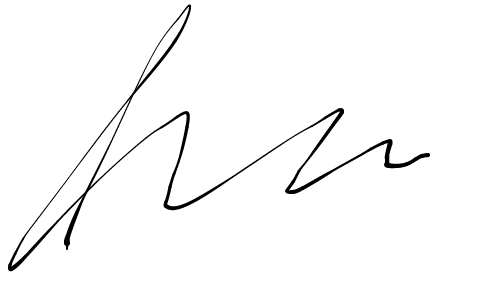
\includegraphics[width=0.35\textwidth]{unterschrift}\vspace*{-0.35cm}
		\\
		\rule[0.5ex]{12em}{0.55pt} & \rule[0.5ex]{12em}{0.55pt} \\
		(Ort, Datum) & (Eigenhändige Unterschrift)
		\\
	\end{tabular*} \\
\end{table}

\end{document}
